\documentclass[tikz,border=3pt]{standalone}
\usepackage[T1]{fontenc}
\usepackage{amsmath}
\usepackage{XCharter}
\usepackage[xcharter]{newtxmath}
\usepackage[scaled=.92]{helvet}
\usepackage{pgfplots}
\usetikzlibrary{arrows.meta,positioning,fit,calc,backgrounds,decorations.pathreplacing,patterns}
\usepgfplotslibrary{groupplots,fillbetween}
\pgfplotsset{compat=1.18}
\definecolor{ink}{HTML}{172536}
\definecolor{rgb}{HTML}{3563B8}
\definecolor{event}{HTML}{17857C}
\definecolor{fusion}{HTML}{76529C}
\definecolor{reference}{HTML}{8994A3}
\definecolor{warn}{HTML}{AC5948}
\definecolor{muted}{HTML}{657183}
\definecolor{rule}{HTML}{D9E0E8}
\definecolor{pale}{HTML}{F5F7FA}
\color{ink}
\tikzset{box/.style={rounded corners=2pt,draw=rule,fill=white,align=center,inner sep=4pt,font=\sffamily\fontsize{9}{10.8}\selectfont,minimum height=9mm},rb/.style={box,draw=rgb!50,fill=rgb!5},eb/.style={box,draw=event!50,fill=event!5},fb/.style={box,draw=fusion!55,fill=fusion!5},arrow/.style={-{Latex[length=1.8mm]},line width=.65pt,draw=muted},note/.style={font=\sffamily\fontsize{8.4}{10.2}\selectfont,align=center,text=muted},heading/.style={font=\sffamily\fontsize{10}{12}\selectfont\bfseries,align=left,text=ink}}
\pgfplotsset{paper/.style={width=15.7cm,height=6cm,axis lines*=left,axis line style={rule},tick style={draw=none},tick label style={font=\sffamily\fontsize{8.8}{10.4}\selectfont,text=muted},label style={font=\sffamily\fontsize{9.4}{11}\selectfont,text=ink},title style={font=\sffamily\fontsize{10}{12}\selectfont\bfseries,text=ink},legend style={draw=none,fill=none,font=\sffamily\fontsize{9}{11}\selectfont,cells={anchor=west}},grid=major,grid style={rule!65,line width=.3pt},minor tick num=0,scaled ticks=false,unbounded coords=jump,clip mode=individual}}
\begin{document}

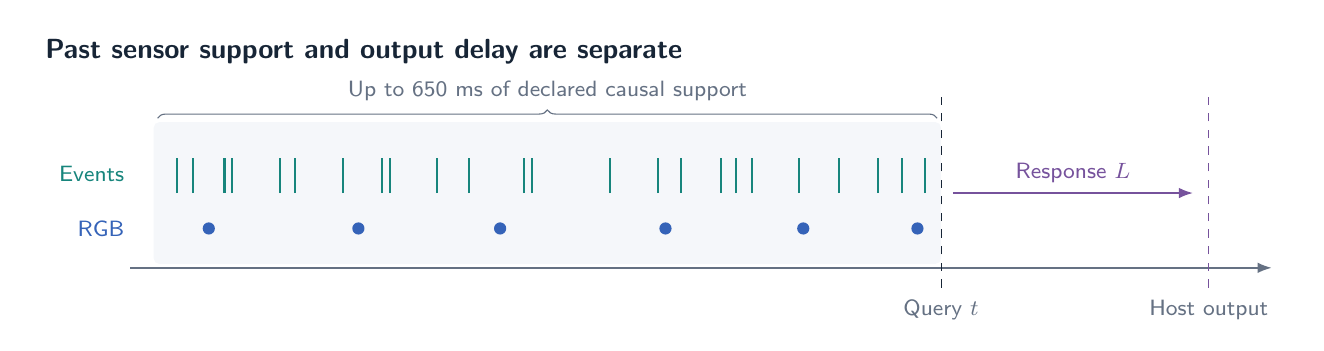
\begin{tikzpicture}[x=1cm,y=1cm]
\path[use as bounding box] (0,-.25) rectangle (16.1,3.5);
\node[heading,anchor=west] at (.1,3.2) {Past sensor support and output delay are separate};
\fill[pale,rounded corners=2pt] (1.6,.5) rectangle (11.6,2.3);
\draw[arrow] (1.3,.45)--(15.8,.45);
\draw[dashed,ink] (11.6,.2)--(11.6,2.7);
\draw[dashed,fusion] (15,.2)--(15,2.7);
\node[note,anchor=east,text=event] at (1.35,1.65) {Events};
\node[note,anchor=east,text=rgb] at (1.35,.95) {RGB};
\foreach \x in {1.9,2.1,2.5,2.6,3.2,3.4,4.0,4.5,4.6,5.2,5.6,6.3,6.4,7.4,8.0,8.3,8.8,9.0,9.2,9.8,10.3,10.8,11.1,11.4}{\draw[event,line width=.75pt] (\x,1.4)--(\x,1.85);}
\foreach \x in {2.3,4.2,6.0,8.1,9.85,11.3}{\fill[rgb] (\x,.95) circle (2.2pt);}
\draw[decorate,decoration={brace,amplitude=3pt},muted] (1.65,2.35)--(11.55,2.35);
\node[note] at (6.6,2.7) {Up to 650 ms of declared causal support};
\draw[arrow,fusion] (11.75,1.4)--node[above,note,text=fusion]{Response \(L\)}(14.8,1.4);
\node[note] at (11.6,-.08) {Query \(t\)};
\node[note] at (15,-.08) {Host output};
\end{tikzpicture}
\end{document}
